%!TEX root = ../../main.tex

\chapter{Grundlagen}
\label{chapter:3}

% TODO: kleiner Einleitungstext schreiben

\section{Humanzentriertes Design}

Beim Entwickeln neuer Software setzen erfahrene Softwareentwickler häufig auf einen gut durchdachten Plan und Struktur. Dabei wird auf bestimmte Entwicklerprozesse gesetzt. Einer der bekanntesten Prozesse in der Softwareentwicklung ist hierbei der “Software Development Lifecycle” (kurz: SDLC). Der SDLC wird genutzt, um möglichst effiziente, kostengünstige Software mit hoher Qualität zu designen, entwickeln und produzieren.\cite{shylesh:2017} Es gibt eine Menge verschiedene Modelle des SDLC, jedoch haben alle Modelle im Grunde dieselbe Struktur: Planen - Designen - Implementieren - Testen. Besonders auf den Baustein “Design” soll in diesem Kapitel tiefer eingegangen werden.

Eine der weitverbreitetsten Designmodelle ist das “Human Centered Design” (kurz: HCD, dt.: menschenzentriertes Design).  Dabei handelt es sich um eine Designtechnik, bei der der Mensch im Vordergrund des Entwicklungsprozesses steht.\cite{hbsc:2020} Laut der Webseite der Harvard Business School liegen die Ziele des HCD darin, die Ziele, Wünsche und Vorlieben des Produktnutzers stetig im Auge zu behalten.\cite{hbsc:2020} Dort beschreibt ein Dekan der Harvard Business School vier grundlegende Phasen im HCD. Diese sind laut Dekan Srikant Datar folgende Phasen: Clarify - Ideate - Develop - Implement.\cite{hbsc:2020} Wiederum definiert Sim van der Ryn in seinem Paper “Human Centered Design” aus dem Jahr 2013 das Vorgehen des HCD ein wenig anders, jedoch ähnlich. Dieser schreibt, dass man sich zuerst mit dem potenziellen Nutzer beschäftigen sollte.\cite{vanderryn:2013} Anschließend wird das Problem definiert, eine Idee erarbeitet, ein Prototyp erstellt und abschließend getestet.\cite{vanderryn:2013}

\begin{figure}[h]
    \centering
    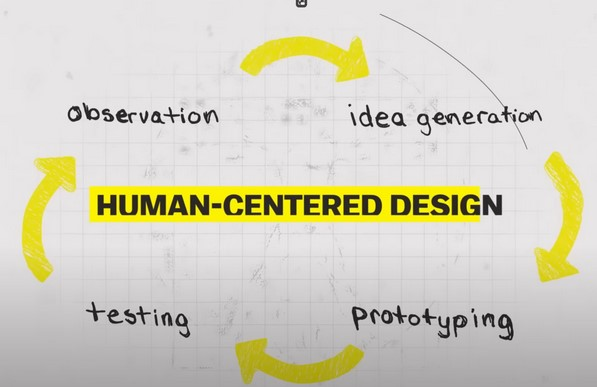
\includegraphics[width=1\textwidth]{images/03/HCD.jpg}
    \caption{Humand Centered Design Prozess}
\end{figure}

Zu den Vorteilen des HCD gehören unter anderem eine hohe Nutzerzufriedenheit, da die Meinung von Personen unmittelbaren Einfluss auf das Design des Produkts nehmen und so sicherstellen, dass alle Bedürfnisse und Erwartungen an das Produkt garantiert werden. Zudem kann dadurch auf die Wechselwirkung zwischen Menschen und Objekten besser verstanden werden, da man durch die Designfrage wichtige Erkenntnisse über das Verhalten bzw. Bedürfnisse der Menschen oder zumindest einer Personengruppe bekommt.

% ! Problem with Quote
% Zu den Vorteilen des HCD gehören unter anderem eine hohe Nutzerzufriedenheit, da die Meinung von Personen unmittelbaren Einfluss auf das Design des Produkts nehmen und so sicherstellen, dass alle Bedürfnisse und Erwartungen an das Produkt garantiert werden.\cite{hcd:2021} Zudem kann dadurch auf die Wechselwirkung zwischen Menschen und Objekten besser verstanden werden, da man durch die Designfrage wichtige Erkenntnisse über das Verhalten bzw. Bedürfnisse der Menschen oder zumindest einer Personengruppe bekommt.\cite{let:2022}

% ! Here too
Jedoch gibt es auch einige Nachteile bzw. Probleme des HCD. Ein Aspekt wäre die rapide Produktlebenszyklus. Durch die ständig wechselnden Bedürfnisse und Anforderungen an ein Produkt, stehen Designer und Designteams ständig unter großen Herausforderungen, um die Ansprüche treffen zu können. Häufig könnten aber auch eben diese menschlichen Anforderungen an ein Produkt zum Problem werden, da diese Anforderungen nicht umsetzbar und realisierbar sind.\cite{pod:2016}

\section{Nutzerzentriertes Design}

Achtet man nun beim Entwickeln neuer Software besonders auf den Nutzer und baut diese nach seinen Wünschen und Anregungen auf, so spricht man in diesem Fall von Nutzerzentriertem Design (kurz: UCD). Der wesentliche Unterschied zum Menschenzentrierten Design (HCD) ist jedoch, dass das Nutzerzentrierte Design soziale und kulturelle Aspekte nicht mit in das Design einfließen lässt.\cite{hcd2:2021} Diese Aspekt spielen beim Menschenzentrierten Design eine wesentliche Rolle. Dennoch wird UCD heutzutage auch mit HCD gleichgestellt.\cite{ucd1:2011}

Einer der zentralen Aspekte beim UCD sind so genannte Personas. Laut dem Buch "Persona Design in Participatory Agile Software Development" werden Personas häufig als Methode im UCD genutzt, um fiktionale Charaktere zu erschaffen, die verschiedene Nutzer bzw. gesamte Nutzergruppen zu repräsentieren.\cite{personaDesign:2020} Eine Persona wird dabei meistens in einer Erzählung beschrieben.\cite{ucd1:2011} Das Ziel liegt laut dem Artikel "Personas and user-centered design: How can personas benefit product design processes?" darin, die Persona wie eine reale Person darzustellen und die Bedürfnisse der Persona anschaulich innerhalb einer Gescichte darzustellen, um diese in die Entwicklung des Produktes einfließen zu lassen.\cite{ucd1:2011}
Grundsätzlich startet eine solche Erzählung mit einer Beschreibung der Person.\cite{ucd1:2011} Während der Beschreibung werden wichtige charakteristische Merkmale der Persona, wie z.B. Vorlieben und Abneigungen, Beruf etc. eingegangen.\cite{ucd1:2011}

\subsection{Erstellen einer Persona}
Die Erstellung einer Persona zählt zu den wesentlichen Punkten im UCD. In einem wissenschaften Paper der Universität Rostock wird der Bildungsprozess einer Persona beschrieben. Der komplette Entwicklungsprozesse einer Persona ist ebenfalls in der nachfolgenden Abbildung dargestellt:

\begin{figure}[h]
    \centering
    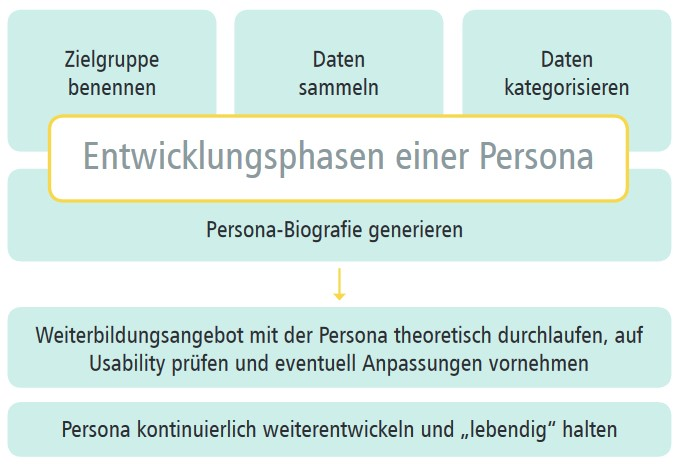
\includegraphics[width=1\textwidth]{images/03/entwicklungPersona.jpg}
    \caption{Entwicklungsprozess Persona \cite{personamethode}}
\end{figure}

Zu sehen ist, dass nahezu alle Schritte, welche vor der Erstellung von Personas passieren, mit Daten zutun haben. Besonders das Sammelen und Kategorisieren der Daten wird hier thematisiert.\cite{personamethode} Dazu schreibt der Wissenschaftler Frank Ploß in seiner Diplomarbeit "Usability Engineering in einem Open-Source-Projekt", welches ebenfalls von der Universität Rostock zitiert wird, dass es sich bei den eizenlenen Designstufen um iteratives Modell handelt.\cite{osp:masterthesis}
Das bedeutet im Grunde genommen nur, dass die einzelnen Schritte aufeinandner aufbauend sind. In dem Artikel wird zudem erwähnt, dass bereits im Vorfeld der Personaentwicklung Fragen über die Zielgruppe gestellt werden sollen, um die Erschaffung einer Persona zu vereinfachen.\cite{personamethode}
Diesen Schritt wird im Rahmen der Studienarbeit ausführlicher im Rahmen einer Umfrage durchgeführt.

Nachdem Sammeln und Kategorisieren der Daten wird die Persona definiert.\cite{personamethode} In diesem Schritt wird laut dem wissenschaftlichen Artikel der Universität Rostock eine Art Kurzbiografie für jede Persona erschaffen.\cite{personamethode} Als Beispiel für eine Persona in der Praxis verwendet die Universität Rostock deshalb Steckbriefe, um ihre Personas so kurz wie möglich, mit möglichst vielen Informationen darzustellen.\cite{personamethode}

Zum Abschluss sollten die Personas noch einen so genanntes Weiterbildungsangebot durchlaufen. Das bedeutet, dass man sich beispielsweise in die Sicht eines Kunden versetzt und als die gerade eben erstellte Persona den Einkaufsprozess durchläuft.\cite{personamethode} Dieser Schritt hilft dabei, die Persona noch stärker zu definieren und evtl. Schwächen/Stärken herauszufinden.

\section{Einführung in die Webentwicklung}

Die Webentwicklung ist ein sehr großer Bereich der Softwareentwicklung und umfasst die Entwicklung von Webanwendungen, die auf den aktuellsten Technologien, Frameworks und Tools basieren. Die Schaffung zeitgemäßer Webanwendungen beinhaltet verschiedene Aspekte, von der Frontend-Entwicklung bis zur Back-End-Entwicklung und der Nutzung von \acf{API}s und Datenbanken.

Der Standard für die Webentwicklung ist die Verwendung von JavaScript, \acf{HTML} und \acf{CSS}. Diese Technologien sind die absoluten Grundlagen für die Entwicklung von Webanwendungen, auf denen alles Weitere aufbaut.

Die Frontend-Entwicklung von Webanwendungen umfasst hierbei die Verwendung von Frameworks wie React, Angular und Vue. Diese wiederum basieren auf der Programmiersprache JavaScript und ermöglichen die Erstellung von wiederverwendbaren Komponenten, auch bekannt als Komponentenarchitektur. Die Verwendung von Frameworks ermöglicht darüber hinaus auch die Anwendung moderner Entwicklungspraktiken wie Komponententests, Test-Driven-Development und Continuous Integration. Die Verwendung von Frameworks ermöglicht es Entwicklern, die Entwicklungseffizienz zu verbessern und die Wartbarkeit der Anwendung zu erhöhen. Die zuvor angesprochenen Frameworks sind nur einige der vielen Frameworks, die existieren. Es gibt eine Vielzahl von Frameworks, die alle ihre eigenen Stärken und Schwächen haben. Die Wahl des richtigen Frameworks hängt von den Anforderungen des Projekts ab und sollte sorgfältig abgewogen werden, um die beste Benutzererfahrung zu gewährleisten.\cite{modern-webdevelopment:1, modern-webdevelopment:2}

\subsection{Programmiersprache JavaScript}

JavaScript ist eine interpretierte Programmiersprache, welche hauptsächlich Anwendung bei Webanwendungen findet. Sie wird dafür genutzt, um Interaktionen als auch die dynamische Veränderung auf der Webseite zu ermöglichen. Dadurch kommt JavaScript größtenteils im Browser vor, also auf der Seite des Clients. JavaScript kann neben dem sehr verbreiteten objektorientierten Programmierstil auch als prozedurale Programmiersprache eingesetzt werden, dadurch ist JavaScript sehr flexibel, was einerseits vorteilhaft ist, aber auch zum Nachteil führt, da es keine konkreten Richtlinien gibt, woran man sich halten sollte. Aber JavaScript ist nicht nur im Programmierstil sehr flexibel, denn dadurch, dass es nur eine interpretierte Programmiersprache ist, besitzt es weitere Nachteile gegenüber von kompilierten Sprachen.

Einer der größten Nachteile hierbei ist, dass es bei JavaScript keine direkte Typisierung gibt, die im Vorhinein im Quellcode festgelegt wird, wie bei typisierten Programmiersprachen wie z. B. Java. Dadurch können theoretisch jegliche Art von Daten in einer Variable gespeichert werden. Das führt dazu, dass man während des Entwicklungsprozesses einfache Fehler nicht festgestellt werden können, sondern erst bei dem Ausführen der Software. Bei Programmiersprachen, welche typisiert sind, kann dieses Problem schon im Vorhinein festgestellt werden, und dadurch einfache Fehler wie z. B. das Datentype nicht miteinander übereinstimmen, ob auf diese Variable in diesem Kontext zugegriffen werden kann oder dass eine Variable nicht existiert, bereits im Vorhinein festgestellt werden. Dazu kommt, dass neben den nicht typisierbaren Variablen in JavaScript die Eingabe- und Ausgabeparameter einer Funktion nicht typisieren kann. Diese Tatsache führt häufig zu Fehlern, welche erst im laufenden Betrieb der Software festgestellt werden können. Dadurch wird JavaScript-Code sehr schwer wartbar, da Entwickler beim Lesen des Quellcodes nicht genau wissen können, was in einer Variable gespeichert ist und was die Funktionen genau machen. Um den Quellcode letztlich korrekt zu verstehen, ist es nötig, sich intensiv einzuarbeiten, was sowohl viel Zeit, als auch Geld kostet.

Im Folgenden ist ein kleines Beispiel, wie sich JavaScript von Java unterscheidet hinsichtlich der Typisierung von der Deklaration von Variablen und Funktionen.

\begin{lstlisting}[caption=Java Variablen und Funktion deklarations Beispiel, label=variables-and-functions-example-java, language=Java]
    // Deklaration von Typisierten Variablen
    int name = 1;
    char name = "c";
    String name = "John";

    // Deklaration von Typisierten Funktionen
    private int add(int a, int b) {
        return a + b;
    }
\end{lstlisting}

\begin{lstlisting}[caption=JavaScript Variablen und Funktion deklarations Beispiel, label=variables-and-functions-example-javascript, language=JavaScript]
    // Deklaration von Variablen
    let a = 1;
    let b = "c";
    let c = "John";

    // Deklaration von Funktionen
    function add(a, b) {
        return a + b;
    }
\end{lstlisting}

Grundsätzlich ist es in JavaScript nicht möglich direkt zu wissen, was in einer Variable sein kann, schon bei einfachen Funktionen wie einer Additionsfunktion wird in der JavaScript-Variante nicht direkt deutlich, dass eine Zahl zurückkommen soll. Den es wäre auch möglich einen zusammengefügten String zurückzugeben. Bei Java hingegen wird schnell deutlich, was genau Funktionen machen sollen. Dennoch hat JavaScript seine Vorteile, welcher hauptsächlich in der Erlernbarkeit der Sprache liegt. Ein einfaches „Hallo Welt“ Beispiel ist zügig geschrieben. Wenn man das z. B. mit Java vergleicht, gibt es wesentlich mehr zu verstehen, als auch zu schreiben.

\begin{lstlisting}[caption=„Hallo Welt“ Beispiel in Java, label=hello-world-example-in-java, language=Java]
public class HelloWorld {
	public static void main (String[] args) {
		System.out.println("Hello World!");
	}
}
\end{lstlisting}

\begin{lstlisting}[caption=„Hallo Welt“ Beispiel in JavaScript, label=hello-world-example-in-javascript, language=JavaScript]
    console.log("Hallo Welt");
\end{lstlisting}

Wie schon zuvor erwähnt, ist die objektorientierte Programmierung sehr verbreitet und dadurch auch ein Standard. JavaScript hingegen verwendet eine sehr abstrakte Implementation von Objekten, was das objektorientierte Programmieren erschwert, um jedoch in JavaScript objektorientierte zu programmieren, wird die Flexibilität der Sprache genutzt, um sich eine eigene Struktur zu bauen. Durch diese abstrakte Implementation von Objekten, ist jede Variable, egal ob String, Zahl oder Funktion ein Objekt. Jedoch existieren Konzepte wie Klassen, Vererbung und Zugriffsbeschränkung nicht direkt. Über Umwege können Klassen und Vererbungen mittlerweile realisiert werden.

JavaScript ist in dieser Arbeit von Relevanz, da jedes Frontend Framework welche in späteren Abschnitten angesprochen wird darauf basiert und diverse Konzepte von JavaScript verwendet. Zudem ist JavaScript die einzige Programmiersprache, welche im Browser ausgeführt werden kann. Das bedeutet, dass JavaScript die einzige Programmiersprache ist, welche direkt mit dem Nutzer interagieren kann. Das ist ein großer Vorteil, da dadurch die Interaktion mit dem Nutzer direkt im Browser stattfinden kann, ohne dass der Browser die Webseite neu laden muss. Dadurch können Webanwendungen wie die CO2-Runter-App eine bessere Nutzererfahrung bieten, da die Interaktion mit dem Nutzer schneller und flüssiger ist. Eine detailliertere Beschreibung von JavaScript findet man auf der Mozilla Developer Network JavaScript Webseite.\cite{javascript}

\subsection*{JavaScript XML}

% TODO: das vlt noch ein wenig erklären weil wegen React vermutlich viel JSX im Code auftreten wird ? kann man aber auch später machen

\subsection{Komponentenarchitektur}

% TODO: ausarbeiten

\subsection{Frontend Frameworks}

Die Frontend-Entwicklung spielt eine entscheidende Rolle bei der Gestaltung der Benutzeroberfläche und der Benutzerinteraktion, welche wiederum Hand in Hand mit der Nutzer Zentrierten Design eingeht. Es gibt verschiedene Frameworks, die Entwicklern helfen, leistungsstarke und ansprechende Benutzeroberflächen zu erstellen. Drei der prominentesten Frontend-Frameworks sind:

% TODO: mehr in Detail ausarbeiten für die Frameworks ?, vlt ansprechen das man SPA macht und das es client seitiges Rendering ist

\begin{itemize}

    \item \textbf{Angular:} Angular ist ein von Google entwickeltes TypeScript-basiertes Framework. Es bietet eine umfangreiche Sammlung von Werkzeugen und Bibliotheken, die Entwicklern helfen, dynamische Single-Page-Anwendungen zu erstellen. Die Struktur von Angular erleichtert die Organisation des Codes und bietet eine klare Trennung von Logik und Darstellung.\cite{angular}

    \item \textbf{Vue:} Vue.js ist ein progressives JavaScript-Framework, das sich durch seine leichte Integration, Flexibilität und eine sanfte Lernkurve auszeichnet. Es ermöglicht die Erstellung interaktiver Benutzeroberflächen und wird von einer aktiven Community unterstützt, die ständig zur Weiterentwicklung und Verbesserung beiträgt.\cite{vuejs}

    \item \textbf{ReactJS:} React, entwickelt von Facebook, ist eine beliebte JavaScript-Bibliothek, die sich auf die Erstellung wiederverwendbarer \acf{UI}-Komponenten konzentriert. Durch die Verwendung von \acf{JSX} können Entwickler eine hierarchische Struktur aufbauen, die zur Erstellung dynamischer Benutzeroberflächen beiträgt.\cite{reactjs}

\end{itemize}

% TODO: Tabelle mit den Frameworks und deren Eigenschaften, besser übersetzen und anpassen

% ! Tabellen Format ist im Dokument ein wenig verschoben!!! das noch fixen

\begin{longtable}{@{\extracolsep{\fill}}|c|c|c|c|@{}}
    \hline
    \multicolumn{1}{|c|}{\textbf{Parameter}} &
    \multicolumn{1}{c|}{\textbf{Angular}}    &
    \multicolumn{1}{c|}{\textbf{ReactJS}}    &
    \multicolumn{1}{c|}{\textbf{Vue}}                                                                   \\ \hline
    \endfirsthead
    \hline
    \multicolumn{1}{|c|}{\textbf{Parameter}} &
    \multicolumn{1}{c|}{\textbf{Angular}}    &
    \multicolumn{1}{c|}{\textbf{ReactJS}}    &
    \multicolumn{1}{c|}{\textbf{Vue}}                                                                   \\ \hline
    \endhead

    \hline
    \multicolumn{4}{|r|}{{Die Fortsetzung erfolgt auf der nachfolgenden Seite}}                         \\ \hline
    \endfoot

    \endlastfoot
    Unterstützung                            & Google     & Facebook             & Community            \\ \hline
    Typ                                      & Framework  & Bibliothek           & Framework            \\ \hline
    Größe                                    & Mittel     & Klein                & Sehr klein           \\ \hline
    Sprache                                  & TypeScript & JavaScript           & JavaScript           \\ \hline
    Leistung                                 & Gut        & Gut                  & Gut                  \\ \hline
    Datenbindung                             & Beide      & Einfach              & Einfach              \\ \hline
    Lernkurve                                & Steil      & Einfach              & Einfach              \\ \hline
    Nutzung                                  & 2.         & 1.                   & 3.                   \\ \hline
    Entwicklungszeit                         & Mittel     & Relativ kurz         & Schnell              \\ \hline
    Entwicklungsgeschwindigkeit              & Mittel     & Schnell              & Schnell              \\ \hline
    Am besten geeignet für                   & PWA, SPA   & E-Commerce, PWA, SPA & Schnelle Entwicklung \\ \hline
    \caption{Vergleich von Angular, Vue und ReactJS \cite{angular-vuejs-reactjs-comparison:1, angular-vuejs-reactjs-comparison:2}}
    \\
\end{longtable}

% TODO: die Quellen vlt nochmal anschauen und ein besseres Fazit schließen können!!

Diese Frameworks haben jeweils ihre eigenen Stärken und eignen sich für unterschiedliche Projekte je nach Anforderungen, Teampräferenzen und Zielen.\cite{angular-vuejs-reactjs-comparison:3, angular-vuejs-reactjs-comparison:4}

Für die CO2-Runter-App wurde ReactJS als Frontend-Technologie ausgewählt, aufgrund seiner Flexibilität, Leistung und der großen Unterstützung durch die Entwickler-Community. ReactJS ermöglicht die Entwicklung einer reaktionsfähigen Benutzeroberfläche, die schnell und effizient auf Änderungen reagiert.

Zusätzlich zur Verwendung von ReactJS könnte die Anwendung einer \acs{UI}-Bibliothek wie beispielsweise Material-UI oder Ant Design die Entwicklung beschleunigen. Diese Bibliotheken bieten vorgefertigte Komponenten und Stile, die nahtlos in ReactJS integriert werden können, um die Entwicklung zu vereinfachen und ein konsistentes Erscheinungsbild zu gewährleisten.

Die Kombination von ReactJS mit einer solchen \acs{UI}-Bibliothek erleichtert die Implementierung von Designelementen und trägt zur konsistenten Gestaltung der Anwendung bei, während gleichzeitig die Entwicklungseffizienz verbessert wird.

\section{Werkzeuge}
\label{chapter:3-werkzeuge}

Beim Weiterentwickeln der CO2-Runter-App werden zahlreiche Tools genutzt, um die Entwicklungsumgebung zu verbessern und die Entwicklung zu vereinfachen. Da jedoch einige Tools auf das Backend und die Datenbank bezogen sind, werden diese außen vor gelassen. Es wird ausschließlich auf diejenigen eingegangen, die für das Frontend relevant sind. Diese Tools sind wichtig für die Weiterentwicklung der CO2-Runter-App und spielen auch für das nutzerzentrierte Design eine Rolle.

\subsection{NPM - Node Package Manager}
\label{chapter:3-werkzeuge-npm}

\acs{NPM} ist die Abkürzung für \acf{NPM}. Wie der Name schon beschreibt, ist NPM ein Paketmanager, der bei der Installation von Node.js mitgeliefert wird. Er ermöglicht somit die Installation und Verwaltung von JavaScript-Paketen.

Ein Paketmanager ist eine Software, die es ermöglicht, sogenannte Pakete herunterzuladen und in ein Projekt zu importieren. Unter einem Paket versteht man ein Projekt, das von einem Entwickler bereitgestellt wurde, um von anderen Entwicklern in deren Projekten eingebunden zu werden. Auf diese Weise können Entwickler ihre Arbeit miteinander teilen und Zeit sparen, indem sie bereits vorhandene Projekte verwenden, anstatt alles von Grund auf neu entwickeln zu müssen.

Für jeden Paketmanager gibt es eine Paketzentrale oder auch Registry genannt. In der Registry von \acs{NPM} sind über 800.000 Pakete/Projekte zu finden. \acs{NPM} ermöglicht außerdem, eine bestimmte Version eines Pakets in ein Projekt zu importieren. Diese Funktion erlaubt es einem Entwickler, selbst mit veralteten Versionen eines Projektes weiterzuarbeiten. \acs{NPM} ist nur einer von vielen Paketmanagern, die es gibt, dennoch hat sich \acs{NPM} im JavaScript-Umfeld als das Standardwerkzeug für die Paketverwaltung herausgebildet.\cite{npm}

% TODO: weitere Packetmanager aufführen, Bun, PNPM, Yarn ?

\subsection{Material UI (MUI)}
\label{chapter:3-werkzeuge-mui}

Das letzte Werkzeug ist \acf{MUI}. Es ist letztlich eine Bibliothek von unterschiedlichen Web-Komponenten, zum Beispiel Knöpfe, Textfelder etc., die einem Entwickler ermöglichen, schnell und einfach eine schöne und moderne Benutzeroberfläche zu erstellen. \acs{MUI} ist dabei eine \acs{UI}-Komponenten-Bibliothek, die auf ReactJS basiert und die Material Design Richtlinien von Google anwendet, um ein einheitliches, schönes modulares Design zu schaffen, und somit die Entwicklung von Webanwendungen oder Prototypen zu vereinfachen.\cite{materialui}

% TODO: weiter schrieben und verweiß auf das nächste kapitel oder so ?
